
\section{Fachliche Grundlagen}

Dieses Kapitel beschäftigt sich vor allem mit Quellcode.
Wie er erstellt wird, wie er aussieht und welche Entwicklungen es dabei gegeben hat.
Danach kommen wir zu ansätzen Quellcodes zu strukturieren und ihn lesbar zu gestallten.

\subsection{Quellcode und der Author}

Quelltext ist eine für den Computer verständliche Form
eines arbeitsablaufes. Er kann durch einen Kompiler in Maschienencode übersetzt werden.
In den meisten fällen ist er in Textform verfasst und für einen Menschen lesbar.

In einem Softwareprojekt ist er die detailierteste Spezifikation der zu erstellenden
Software und all ihrer Komponenten. Alles wir in ihm so eindeutig beschrieben
das ein Computer diesen umsetzen kann. Die Modell getriebene Entwicklung, vor allem
UML, ist für die direkte Übersetzung in Maschienencode aus heutige Sicht nicht geeignet
da an dieser stelle implementierungsdetails verloren gehen. \cite[S. 26]{Martin}

Der Author des Quelltextes ist der Programmierer. Seine Aufgabe ist es
die Spezifikation zu schreiben.

\subsection{Wandel in der Entwicklung von Quelltexten}

In den anfängen des Computerzeitalters war der Programmierer meistens der einzige
Leser seiner Programme. Hauptaugenmerk lag auf der Funktion es Programmes
und dem effizienten Umgang mit den Ressourcen. Damals gab es noch keine
Objekt orientierten Sprachen. Zudem waren die Arbeitsumgebungen der Entwickler
wesentlich bescheidener als in der heutigen Zeit. Quelltexte wurden im ASCII-Code
Kodiert und die Bildschirme waren nur 80 Zeichen breit.

Durch technische Entwicklungen wie z.B. das Internet, größere Bildschirme und
immer leistungsfähigere Computer. Mitlerweile gibt es für die meisten Sprachen
eine sehr gute Toolunterstützung für den Programmierer. Moderne IDEs gehen
 itlerweile über Syntaxhighlighting hinaus. Funktionen wie automatische Code
Vervollständigung gehören mitlerweile zum Standard.

Das Internet bietet dem Entwickler eine schnelle Möglichkeit nach Lösungen und
ansätzen für Probleme oder einfach der entsprechenden Dokumentation zu suchen.

\subsection{Programmarten}

Die vielzahl von verschiedenen Programmen lassen sich im Kontext dieser Arbeit in
drei Kategorien einordnen.

Als erstes existieren kleine Programme oder Skripte, die für den einmaligen
Gebrauch bestimmt sind. Eine einmalige Migration von daten in ein bestehendes
oder neues System gehört zum Beispiel dazu. Diese Programme haben nur einen
geringen (Quellcode-)Umfang und sind daher einfach zu überschauen.
Da sie auch nur einmalig angewand werden ist der Author zugleich auch der
einzige Leser.

Zur zweiten Kategorie gehören Programme aus der Lehre. Diese haben meist eine
deutlich höhere Dichte an Kommentaren als es für einen Quellcode der anderen
beiden Kategorien der fall ist. Für eine andere Art von Quelltext wäre diese
vielzahl von Kommentaren sogar hinderlich, da sie im extremfall die funktionsweiße
der nächsten Zeile erklärt.

Die dritte Kategorie sind all die Anwendungen die eine längere Zeit im Einsatz sind.
Sie werden häufig nicht von einem Entwickler erstellt sondern von einem ganzen Team.
Dieses führt weiterentwicklungen durch und wartet die Software.
Diese ist die Kategorie an die sich diese Arbeit vor allem richtet.
Hier wird der Quelltext von mehreren Entwicklern gelesen und muss von ihnen in
angemessener Zeit verstanden werden.

\subsection{Formatierung von Quelltexten}

Die Formatierung eines Quellcodes mit korrekter Syntax wird durch
sogenannte Whitespaces (nicht sichtbare Zeichen) vorgenommen.
Dazu gehören vorallem Tabulatoren, Leerzeichen und Zeilenumbrüche.

\begin{listing}[H]
    \begin{minted}{c}
#include <stdio.h>
int main(void){printf("Hello World!");return 0;}
    \end{minted}
    \caption{\enquote{Hello World} Programm in C mit minimalen Whitespaces}
    \label{grundlagen:hellocminimal}
\end{listing}

Für einen Compiler machen Whitespaces häufig keinen Unterschied.
Es ist egal ob der Quellcode viele Whitespaces enthält (Listing \ref{grundlagen:helloc})
oder nur minimale (\ref{grundlagen:hellocminimal}).
Der Zeilenumbruch in Zeile 1 im Listing \ref{grundlagen:helloc} ist hier Teil der Syntax.

Für den Entwickler können Whitespaces zur lesbarkeit beitragen. Listing \ref{grundlagen:helloc}
ist für einen Menschen besser verständlich, da sich mit den Whitespaces die Struktur abbilden lässt.

\begin{listing}[H]
    \begin{minted}{c}
#include <stdio.h>

int main(void) {
    printf("Hello World!");
    return 0;
}
    \end{minted}
    \caption{\enquote{Hello World} Programm in C mit Whitespaces}
    \label{grundlagen:helloc}
\end{listing}

Durch Whitespaces lässt sich der Grauwert des Quellcodes beeinflussen.
Der Grauwert ist u.a. ausschlaggebend für den Gesamteindruck und die Lesbarkeit
eines Textes \cite{Beinert}.

\subsection{Namensgebung}

Neben der Syntax gibt es viele Elemente die der Programmierer benennen muss.
Hierzu gehören z.B. Variablen, Funktionen, Methoden, Klassen, Dateien ...
Je nach Programmiersprache stehen hier unterschiedliche Zeichen zur Verfügung.
Die Buchstaben A-Z sowie die Ziffern 0-9 gehören fast immer dazu, sowie die
Sonderzeichen \enquote{-} und \enquote{\_}. Bei modernen Sprachen die UTF-8
zum Codieren verwenden ist es teilweise auch möglich Umlaute zu verwenden.

Für den Computer sind die Namen egal. So genügt es z.B. alle Variablen \enquote{a1},
\enquote{a2}, ..., \enquote{aN} zu benennen. Der Entwickler kann die Namen jedoch interprettieren und
anhand der namen ihre Bedeutung erahnen.

Das Beispieles aus \cite[S. 46-47]{Martin} zeigt, dass Variablennamen dem
Leser helfen können den Code zu interpretieren.
Listing \ref{grundlagen:namingbad} zeigt einen Quelltext deren Funktionsweise
der Leser zwar versteht aber nicht was damit bezweckt wird.

\begin{listing}
    \begin{minted}{java}
public List<int[]> getThem() {
    List<int[]> list1 = new ArrayList<int[]>();
    for (int[] x : theList)
        if (x[0] == 4)
            list1.add(x);
    return list1;
}
    \end{minted}
    \caption{1. Beispiel zu Codenamen aus \cite[S. 46]{Martin}}
    \label{grundlagen:namingbad}
\end{listing}

Listing \ref{grundlagen:naminggood} ist der selbe Quelltext zu sehen.
Es wurde die selbe Einrückung und der selbe Ablauf verwendet. Lediglich
die Variablennamen wurden verändert.

\begin{listing}
    \begin{minted}{java}
public List<int[]> getFlaggedCells() {
    List<int[]> flaggedCells = new ArrayList<int[]>();
    for (int[] cell : gameBoard)
        if (cell[STATUS_VALUE] == FLAGGED)
            flaggedCells.add(cell);
    return flaggedCells;
}
    \end{minted}
    \caption{2. Beispiel zu Codenamen aus \cite[S. 47]{Martin}}
    \label{grundlagen:naminggood}
\end{listing}

Anhand der Namen kann der Leser nun erkennen das die Methode markierte Felder eines Spielfeldes zurückgibt.

\subsection{Coding Conventions}

Um eine einheitliche Formatierung des Quelltextes zu erreichen werden häufig
Vorgaben für die Formatierung des Codes bestimmt. Diese Vorgaben werden
\enquote{Coding Conventions} genannt. Meist behandeln sie die Einrückung von Quelltexten,
Positionierung der Block-klammern, schreibweiße von Variablen und Methoden aber auch
welche Zeichencodierung für den Quelltext verwendet werden soll.

Beispiele für Coding Conventions sind die GNU Coding Standards \cite{GNUCode},
der Linux Kernel Coding Style\cite{KernelCode} oder die Java Code Conventions\cite{javacode}.

Der Inhalt und Umfang von Coding Conventions kann sich dabei stark voneinander
unterscheiden. Der Linux Kernel Coding Style ist z.B. lediglich 4 Seiten lang,
während die GNU Coding Standards 86 Seiten umfassen.

Coding Conventions können für verschiedene Bereiche eingesetzt werden. Sie können für
ein Projekt erstellt werden wie der Linux Kernel Coding Style oder gleich für eine
ganze Programmiersprache wie die Java Code Conventions.

Eine Coding Convention soll dafür sorgen das ein Quelltext einfach lesbar ist
und er von anderen Entwicklern schnell verstanden und verändert werden kann.

\subsubsection{Tools zum prüfen auf Coding Conventions}

Wenn man einen Syntaxfehler in seinem Programm hat wird
der Kompiler beim kompilieren eine Fehlermeldung ausgeben.
Auf diese Weiße lässt sich feststellen ob der Entwickler
die Syntaktischen regeln der Programmiersprache befolgt hat.

Der Kompiler findet aber keine verstöße gegen eine bestehende Coding Convention.
Hierfür gibt es Tools, die den Quellcode anhand von definierten Regeln analysieren
und so verstöße gegen eine Coding Convention automatiesiert zu finden.

Ein Beispiel für ein solches Tool ist Checkstyle\footnote{siehe auch: http://checkstyle.sourceforge.net/}.
Es ist auf Java Quellcode spezialisiert und bietet eine Beispielkonfiguration für
die Java Coding Conventions.

\subsection{Schlechter Quellcode}


Wir alle hatten schon mit ihm zu kämpfen, schlechter Quellcode. Robert C. Martin beschreibt in seinem
Buch \cite[S. 27f.]{Martin} die Auswirkungen von schlechtem Code wie folgt: Schlechter Code ist schwer
zu lesen und zu verstehen. Er ist schlecht strukturiert und leitet den Leser im schlimmsten Falle in die Irre.
Die Auswirkung ist eine sinkende Produktivität, zu sehen in Abbildung \ref{grundlagen:produktivitaet}.
Dieses hat verschiedene Gründe. Der Code ist durch seine schlechte Verständlichkeit schwer zu warten und erweitern.
Zudem kommt es so leichter zu Bugs. Der Code begünstigt zudem möglicherweise nicht vorhersehbare Seiteneffekte.

\begin{figure}[H]
	\centering
	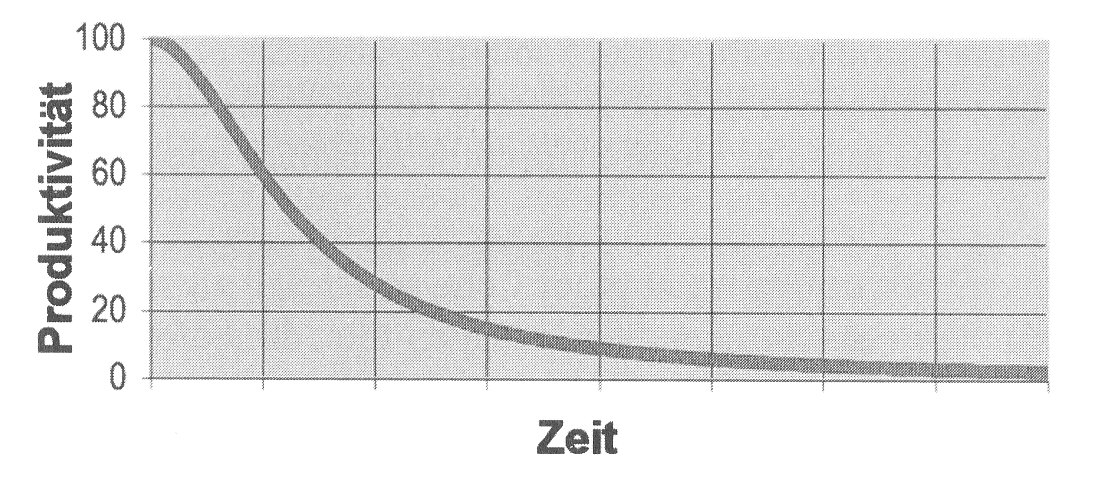
\includegraphics[width=\textwidth]{poduktivitaet.jpg}
	\caption{Produktivität über Zeit aus \cite[S. 29]{Martin}}
	\label{grundlagen:produktivitaet}
\end{figure}

Ein Entwickler der an einem solchen Code arbeitet ist leicht versucht selbst schlechten Quelltext zu schreiben,
da dies vermeintlich schneller geht. Das Resultat, der Code wird immer schwerer zu warten und die Produktivität sinkt weiter.
Eine Neuentwicklung der Software kommt aus der Sicht von \cite[S. 29f.]{Martin} nicht in Frage.
Die neue Software muss neben der Weiterentwicklung der alten Entwickelt werden und trotzdem auf denselben Stand kommen.
Dies ist bei großen Softwareprojekten meistens nicht möglich, da eine solche Lösung häufig zu teuer ist.
Als mögliche Lösung führt er an das jeder Entwickler versuchen sollten den Code an den er gearbeitet hat so sauber wie möglich zu hinterlassen.

\subsection{Guter Quellcode}

Guten Quellcode zu schreiben ist etwas womit sich schon viele Entwickler beschäftigt haben\cite{Martin, Green, Spinellis, reed}.
\cite[S. 32f.]{Martin} hat sich mit den Aussagen von verschiedenen erfahrenen Entwicklern zu sauberem Code auseinandergesetzt.
Er kommt zu folgenden Punkten für guten Code:

\begin{itemize}
\item Testbar
\item Geradlinig, man erkennt den Zweck
\item Verständlich, einfach zu durchschauen, erwartungskonform
\item Keine versteckten Absichten
\item Gute Namen
\item Minimale Abhängigkeiten
\item Keine Redundanzen
\item Keine Fehler/Exceptions verstecken
\end{itemize}

Diese Punkte ähneln sehr stark den Design Ideen der Programmiersprache Python\cite{Peters}.
Wie zu erkennen ist findet sich guter Quelltext auf verschiedenen Ebenen wieder.
Auf unterster Ebene im Quelltext bis hin zum gesamtdesign der Software.
Häufig gehört allerdings ein hohes Maß an Erfahrung dazu einen guten Quelltext zu schreiben.

\subsection{Art and Science}

In vielen Artikeln zu dem Thema finden man die Wörter \enquote{Art} und \enquote{Science}. So z.B.
\enquote{Coding Guidlines: Finding the Art in Science} von \cite{Green} oder \enquote{Science and Art} von \cite[669]{Knuth}.
Damit spielt man darauf an das manche Quelltexte sich so schön lesen und verstehen lassen das sie Kunst sind.
\cite[S. 669]{Knuth} zeigt das nicht nur die Informatik Art und Science in dieser weiße benutzt.
Er fand es auch in einem Buch über die Grundlagen der Photographie und in der Einleitung eines Wörterbuches\cite[S. 669]{Knuth}.
Er zeigt zudem einen Wandel in der Verwendung des Wortes \enquote{Art}.
Früher war es üblich von einem gut ausgeführten Handwerk als Kunst zu reden.
Knuth zieht den Schluss das \enquote{Science} das Wissen ist und \enquote{Art} das angewandte wissen.
In unserem Fall ist das Programmieren das Handwerk und guter Quellcode die Kunst.
Weiterhin hat jeder Programmierer seinen eigenen Stil einen Quellcode zu schreiben.
Selbst Coding Conventions lassen dem Entwickler genug Freiraum für einen eigenen Schreibstil,
da es nicht möglich ist alles mit ihnen zu definieren.
